\documentclass[tikz,border=2pt]{standalone}
\usepackage{amsmath,amssymb}
\usepackage{tikz}
\usetikzlibrary{arrows.meta}

\begin{document}
% Feasible versus infeasible decision vectors: a point inside the polygon satisfies every
% constraint, a point outside violates at least one.
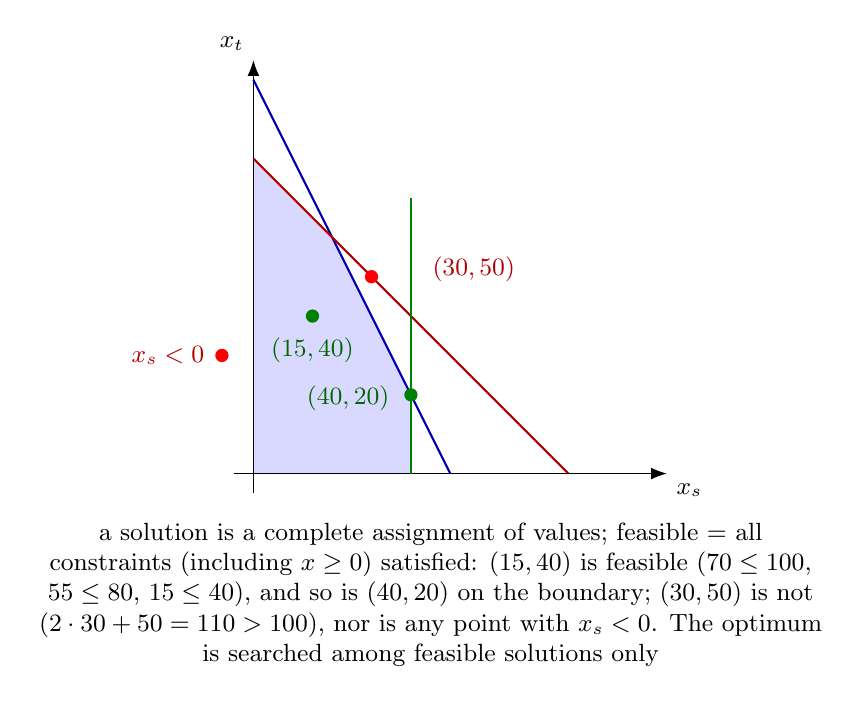
\begin{tikzpicture}[x=0.05cm, y=0.05cm, every node/.style={font=\small}, >={Latex[length=2mm]}]
	\fill[blue!15] (0,0) -- (40,0) -- (40,20) -- (20,60) -- (0,80) -- cycle;
	\draw[->] (-5,0) -- (105,0) node[below right] {$x_s$};
	\draw[->] (0,-5) -- (0,105) node[above left] {$x_t$};
	\draw[blue!70!black, thick] (50,0) -- (0,100);
	\draw[red!70!black, thick] (80,0) -- (0,80);
	\draw[green!50!black, thick] (40,0) -- (40,70);
	\fill[green!50!black] (15,40) circle (2.4pt);
	\node[green!40!black, font=\small, anchor=north] at (15,37) {$(15,40)$};
	\fill[green!50!black] (40,20) circle (2.4pt);
	\node[green!40!black, font=\small, anchor=east] at (37,19) {$(40,20)$};
	\fill[red] (30,50) circle (2.4pt);
	\node[red!70!black, font=\small, anchor=west] at (43,52) {$(30,50)$};
	\fill[red] (-8,30) circle (2.4pt);
	\node[red!70!black, font=\small, anchor=east] at (-10,30) {$x_s<0$};
	\node[anchor=north, align=flush center, text width=10cm] at (45,-10) {a solution is a complete assignment of values; feasible $=$ all constraints (including $x\ge0$) satisfied: $(15,40)$ is feasible ($70\le100$, $55\le80$, $15\le40$), and so is $(40,20)$ on the boundary; $(30,50)$ is not ($2\cdot30+50=110>100$), nor is any point with $x_s<0$. The optimum is searched among feasible solutions only};
\end{tikzpicture}
\end{document}
